
This chapter will introduce Machine Learning (ML) concepts and techniques being explored in this work, namely the classification problem, feature learning, neural networks and encoder and decoder neural networks.

\section{Classification}

In Statistics and Machine Learning, a problem is defined as a classification problem when it consists in identifying to which categories a member of a population belongs to. An example might be identifying which race of domestic cat is shown in a picture containing a cat \cite{Kolla2020}. An algorithm that implements classification is known as a classifier. The classifier works by analysing each observation into dependent variables and either mapping those to the categories or by comparing each observation to previous observations by means of a similarity function or loss function \cite{lorena2021inteligencia}. 

Terminology between Statistics and Machine Learning tend to differ. In this work, we will be using the terminology found in Machine Learning, namely:

\begin{itemize}
	\item dependent variables are called features;
	\item categories are called classes;
\end{itemize}

In this work, we will not focus on a specific classification algorithm since ISA is not dependent on the algorithm used, only on the problem of classification.

\section{Feature learning} \label{sec:feature_learning}

Feature learning, or representation learning\cite{RepLearning}, is a set of techniques that allow a model to discover representations needed for feature detection or classification from raw data. This is a method by which we replace feature engineering and have the model both learn the features and use them to perform the task.

Feature learning can be either supervised, unsupervised or self-supervised:

\begin{itemize}
	\item in supervised learning, features are learned using labeled input data;
	\item in unsupervised learning, features are learned using the relationship between the individual observations in the input data. Examples include principal component analysis and various forms of clustering;
	\item in self-supervised learning, features are learned using unsupervised methods and then input-label pairs are constructed, enabling supervised learning. Examples include autoencoders and word embeddings.
\end{itemize}	

\section{Neural networks}

Neural networks, formally called \emph{artificial neural networks} (ANNs), are computational models inspired by networks of biological neurons \cite{Puri2016}. They are made up of multiple nodes called artificial neurons that map an input to an output based on mathematical operations. This model is used extensively in ML applications because of its perceived intelligent behaviour that comes from the interactions between neurons.

\subsection{Artificial neuron}

The artificial neuron is the most basic block of an ANN. It maps inputs to an output in the given fashion:

\begin{equation} \label{eq:neuron_eq}
	y = f(\mathbf{w} \cdot \mathbf{x} + b),
\end{equation}

where the symbols are defined as:

\begin{equation} \label{eq:neuron_symbols}
	\begin{tabular}{ll}
		$\mathbf{x} = [x_1, x_2, \ldots, x_n]$ & Input vector;\\
		$\mathbf{w} = [w_1, w_2, \ldots, w_n]$ & Weight vector;\\
		$f$ & Activation function; \\
		$y$ & Neuron output; \\
		$b$ & Bias,
	\end{tabular}
\end{equation}

Figure \ref{fig:neuron} shows the artificial neuron model. This model of neuron is useful because it incorporates both the linear combination of input values and bias and the non-linearity of the activation function, which means it may function as a part of an universal function approximator \cite{HORNIK1989}.

\begin{figure}[ht]
	\centering
	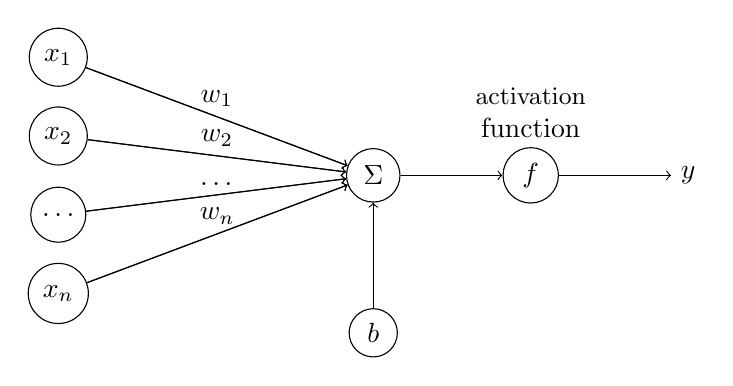
\begin{tikzpicture}
		% Neuron
		\node[circle, draw] (neuron) at (0, 0) {$\Sigma$};
		
		% Inputs
		\foreach \i/\name in {1/$x_1$, 3/$x_2$, 5/$\ldots$, 7/$x_n$} {
			\node[circle, draw] (input\i) at (-4, 4/2-\i/2) {\name};
			\draw[->] (input\i) -- (neuron);
		}
		
		% Weights (above)
		\foreach \i/\name in {1/$w_1$, 3/$w_2$, 5/$\ldots$, 7/$w_n$} {
			\draw[->] (input\i) -- (neuron) node[midway, above] {\name};
		}
		
		% Bias
		\node[circle, draw] (bias) at (0, -2) {$b$};
		\draw[->] (bias) -- (neuron);
		
		% activation function
		\node[circle, draw, label={[align=center]\small activation\\function}] (function) at (2, 0) {$f$};
		\draw[->] (neuron) -- (function);
		
		% Output
		\node (output) at (4, 0) {$y$};
		\draw[->] (function) -- (output);
	\end{tikzpicture}
	\caption{Model of an artificial neuron.} \label{fig:neuron}
\end{figure}

\subsection{The network}

As said before, an ANN is a network of artificial neurons. Such network may be built by having the neurons configured in layers, having each neuron in a layer connected only to neurons in either preceding or following layers or with other arrangement of connections. Figure \ref{fig:fc_nn} shows a simple model of a fully-connected (a neuron in a layer connects to every neuron in the next layer) neural network, having 3 inputs, 4 middle nodes (called a hidden layer) and 3 output nodes.

\begin{figure}[ht]
	\centering
		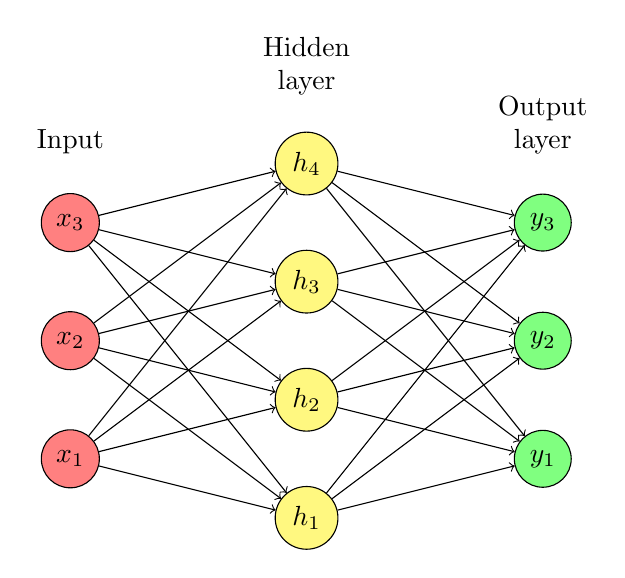
\begin{tikzpicture}[scale=1.5]
			% Input layer
			\foreach \i/\name in {1/$x_1$, 2/$x_2$, 3/$x_3$} {
				\node[circle, draw, fill=red!50] (input\i) at (0, \i) {\name};
			}
			\node[above, align=center] at (0, 3.5) {Input};
			
			% Hidden layer
			\foreach \i/\name in {1/$h_1$, 2/$h_2$, 3/$h_3$, 4/$h_4$} {
				\node[circle, draw, fill=yellow!50] (hidden\i) at (2, \i-1/2) {\name};
			}
			\node[above, align=center] at (2, 4) {Hidden\\layer};
			
			% Output layer
			\foreach \i/\name in {1/$y_1$, 2/$y_2$, 3/$y_3$} {
				\node[circle, draw, fill=green!50] (output\i) at (4, \i) {\name};
			}
			\node[above, align=center] at (4, 3.5) {Output\\layer};
			
			% Connections
			\foreach \source in {1, 2, 3} {
				\foreach \dest in {1, 2, 3, 4} {
					\draw[->] (input\source) -- (hidden\dest);
				}
			}
			
			\foreach \source in {1, 2, 3, 4} {
				\foreach \dest in {1, 2, 3} {
					\draw[->] (hidden\source) -- (output\dest);
				}
			}
		\end{tikzpicture}
		\caption{A model of a simple fully-connected neural network with 3 inputs, 3 outputs and a hidden layer with 4 nodes.} \label{fig:fc_nn}
\end{figure}

\subsection{Learning}

Learning is the process by which an ANN adapts itself to a given task using data. It involves adjusting the weights of the network to improve some predefined metric (e.g. accuracy) and minimizing observed errors. In practice, learning is done by defining a loss function which is evaluated during learning and as long as its output (called loss, for short) decreases, the learning continues.

Most learning models are applications of optimization theory, like the gradient descent algorithm. In this algorithm the purpose is to find a local minima by moving against the gradient of the function. It is the basis for the Adam optimizer \cite{kingma2017adam}, used extensively in ANNs.

\subsubsection{Learning rate}

The learning rate is a parameter in an optimization algorithm, defining the size of each step towards the local minima of a loss function. Higher learning rates shorten the learning time, but at a cost of possibly never converging and higher errors, while setting it at a value too low might have it converging in an undesirable local minimum.

\subsubsection{Backpropagation}

Backpropagation is a method to adjust the weights of the network and minimize the mean squared error. It computes the gradient of the loss function with respects to the weights and propagates backwards from the output layer to the initial layers in order to avoid redundant calculations.

\section{Encoder, decoder and autoencoder neural networks}

Neural networks can be used in feature learning tasks, as shown in section \ref{sec:feature_learning}. We can construct neural networks to learn efficient codings of the input data by means of an encoder network, which is a network that transforms input data into a representation in a latent space. Figure \ref{fig:encoder} shows a representation of an encoder network. A decoder network is much the same as an encoder, but in the opposite direction, transforming the latent space representation into the original data.

\begin{figure}[!ht]
	\centering
	\begin{tikzpicture}
		% Input layer
		\foreach \i in {1,...,10} {
			\node[circle, draw, minimum size=0.8cm] (input\i) at (0, \i) {$x_{\i}$};
		}
	
		% Hidden layers
		\foreach \h in {1,...,6} {
			\node[circle, draw, minimum size=0.8cm, right=of input5] (hidden1\h) at (3, \h * 9 / 7 + 1) {$h_{1,\h}$};
		}
		\foreach \h in {1,...,4} {
			\node[circle, draw, minimum size=0.8cm, right=of hidden16] (hidden2\h) at (6, \h * 9 / 5 + 1) {$h_{2,\h}$};
		}
		\foreach \h in {1,...,2} {
			\node[circle, draw, minimum size=0.8cm, right=of hidden24] (output\h) at (9, \h * 9 / 3 + 1) {$y_{\h}$};
		}
	
		% Connect layers
		\foreach \i in {1,...,10} {
			\foreach \h in {1,...,6} {
				\draw[->] (input\i) -- (hidden1\h);
			}
		}
		\foreach \h in {1,...,6} {
			\foreach \hprime in {1,...,4} {
				\draw[->] (hidden1\h) -- (hidden2\hprime);
			}
		}
		\foreach \h in {1,...,4} {
			\foreach \hprime in {1,...,2} {
				\draw[->] (hidden2\h) -- (output\hprime);
			}
		}
	\end{tikzpicture}
	\caption{Representation of an encoder} \label{fig:encoder}
\end{figure}

An \textbf{autoencoder} is one such networks, composed of two parts: an encoder (or \emph{encoding function} $f$) and a decoder (or \emph{decoding function} $g$) that recreates the data from this representation. The learning problem is then defined as minimizing a loss function $L(\mathbf{x}, g(f(\mathbf{x})))$ that penalizes $g(f( \mathbf{x} ))$ from being too different from $\mathbf{x}$ \cite{Goodfellow-et-al-2016}. A representation of an autoencoder is shown in figure \ref{fig:autoencoder}.

\begin{figure}[!ht]
	\centering
	\begin{tikzpicture}[node distance=3cm, rotate=90]

		% Define block styles
		\tikzstyle{input} = [draw, rectangle, minimum width=1cm, minimum height=3cm, text centered, text width=1cm, fill=blue!20]
		\tikzstyle{encoder} = [draw, trapezium, trapezium stretches=true, trapezium angle=65, minimum width=2cm, minimum height=2cm, text centered, text width=2cm, fill=green!20]
		\tikzstyle{latent} = [draw, circle, minimum size=1cm, text centered, text width=1cm, fill=yellow!20]
		\tikzstyle{decoder} = [draw, trapezium, trapezium stretches=true, trapezium angle=65, minimum width=2cm, minimum height=2cm, text centered, text width=2cm, fill=orange!20]
		\tikzstyle{output} = [draw, rectangle, minimum width=1cm, minimum height=3cm, text centered, text width=1cm, fill=red!20]
		\tikzstyle{arrow} = [thick,->,>=stealth]
		
		% Nodes
		\node (input) [input] {$\mathbf{x}$};
		\node (encoder) [encoder, right of=input, shape border rotate = 270] {Encoder};
		\node (latent) [latent, right of=encoder] {Latent Space};
		\node (decoder) [decoder, right of=latent, shape border rotate = 90] {Decoder};
		\node (output) [output, right of=decoder] {$\mathbf{x}^\prime$};
		
		% Arrows
		\draw [arrow] (input) -- (encoder);
		\draw [arrow] (encoder) -- (latent);
		\draw [arrow] (latent) -- (decoder);
		\draw [arrow] (decoder) -- (output);
		
	\end{tikzpicture}
	\caption{Representation of an autoencoder with input $\mathbf{x}$.} \label{fig:autoencoder}
\end{figure}

It is not useful to have the autoencoder copy each input perfectly to the output. Usually they are restricted in ways that allow them to copy only approximately, and to copy only input that resembles the training data \cite{Goodfellow-et-al-2016}.

One way to restrict the autoencoder is to have the encoder be an undercomplete network, meaning that the dimensionality of the latent space is smaller than the dimensionality of the input space. This forces the autoencoder to learn the most important features of the input data in order to be able to recreate it. In this case, if the decoder is linear and the loss function $L$ is the mean squared error, then the optimal solution to the autoencoder is the principal component analysis \cite{Goodfellow-et-al-2016}. 

Unfortunately, if the encoder and the decoder are allowed too much capacity, the autoencoder will learn to copy the input to the output without learning any useful information about the data distribution \cite{Goodfellow-et-al-2016}. A similar problem occurs if the latent space is allowed to have the same or greater dimension than the input data. 

%A Generative Adversarial Network (GAN) is an architecture for estimating generative artificial intelligence models. It consists of a two-player minimax game between two ANNs: a generative model $G$ and a discriminative model $D$. The purpose of $D$ is to estimate the probability that a sample came from the training data instead of coming from $G$, and the purpose of $G$ is to minimize that probability. A unique solution exists where $D$ outputs the probability of $\frac{1}{2}$ everywhere \cite{Goodfellow2014}. The generator $G$ is, then, not trained to minimize a loss function, but to fool the discriminator $D$. 
%
%We will now be defining some notation for more formal modelling. Let $\mathbf{x}$ be the input data, $D(\mathbf{x})$ is then the output of the discriminator over the input data, which is the probability that the input data came from the training data rather than the generator. For the generator, let $\mathbf{z}$ be a latent space vector sampled from a standard normal distribution. $G(\mathbf{z})$ represents the generator's output, mapping $\mathbf{z}$ to the data space.
%
%$D(G(\mathbf{z}))$ is therefore the probability that a generated input came from the training data. The goal of $G$ is to estimate the distribution which the training data comes from ($p_{data}$) so that it may draw samples from this estimation ($p_G$) \cite{Goodfellow2014}. The minimax loss function will be, therefore :
%
%\begin{equation} \label{eq:minimax}
%	\min_{G} \max_{D} V(D, G) = \mathbb{E}_{\mathbf{x} \sim p_{data}(\mathbf{x})} [\log D(\mathbf{x})] + \mathbb{E}_{\mathbf{z} \sim p_{\mathbf{z}}(\mathbf{z})} [\log(1 - D(G(\mathbf{z})))]
%\end{equation}
%
%In theory, the solution of this game will be when $p_G = p_{data}$ and the discriminator will guess every generated input randomly ($D(G(\mathbf{z})) = \frac{1}{2}$). Figure \ref{fig:gan_flowchart} shows a flowchart of this training model. Algorithm \ref{alg:training_gan} is the training algorithm defined in \citeonline{Goodfellow2014}.
%
%\begin{algorithm}
%	\caption{Minibatch stochastic gradient descent training of GANs as defined in \citeonline{Goodfellow2014}. The number of steps to apply to the discriminator is a hyperparameter $k$.} \label{alg:training_gan}
%	\For{number of training steps}{
%		\For{k steps}{
%			Sample minibatch of $m$ noise samples $[\mathbf{z}^{(1)}, \ldots, \mathbf{z}^{(m)}]$ from noise prior $p_G(\mathbf{z})$; \\
%			Sample minibatch of $m$ examples $[\mathbf{x}^{(1)}, \ldots, \mathbf{x}^{(m)}]$ from data distribution $p_{data}(\mathbf{x})$; \\
%			Update the discriminator by ascending its stochastic gradient: 
%				$$\nabla_{w_D} \frac{1}{m} \sum_{i=1}^{m} \left[ \log D\left( \mathbf{x}^{(i)} \right) + \log \left( 1 - D\left( G\left( \mathbf{z}^{(i)} \right) \right) \right)  \right]; $$
% 		}
% 		Sample minibatch of $m$ noise samples $[\mathbf{z}^{(1)}, \ldots, \mathbf{z}^{(m)}]$ from noise prior $p_G(\mathbf{z})$; \\
% 		Update the generator by descending its stochastic gradient:
% 			$$\nabla_{w_G} \frac{1}{m} \sum_{i=1}^{m} \log \left( 1 - D\left( G\left( \mathbf{z}^{(i)} \right) \right) \right);$$
%	}
%\end{algorithm}
%
%\begin{figure}[ht]
%	\centering
%	\begin{tikzpicture}[node distance=4cm]
%		
%		% Nodes
%		\node[rectangle, draw] (generator) {Generator};
%		\node[rectangle, draw, below of=generator] (discriminator) {Discriminator};
%		\node[left of=generator, align=center] (input) {Random\\Noise};
%		\node[rectangle, draw, right of=discriminator, xshift=3cm, align=center] (output) {Real or\\Fake};
%		\node[left of=discriminator, align=center] (realdata) {Real\\Data};
%		
%		% Arrows
%		\draw[->] (input) -- (generator);
%		\draw[->] (generator) -- (discriminator) node[midway, left, align=center] {Generated\\Data};
%		\draw[->] (discriminator) -- (output) node[midway, above] {Discriminator Score};
%		\draw[->] (output) -- (generator) node[midway, above, fill=white] {Backpropagation};
%		\draw[->] (output.south west) to[out=240, in=300]  node[anchor=north, midway] {Backpropagation} (discriminator.south east);
%		
%		% Dashed line
%		\draw[dashed, ->] (realdata) -- (discriminator);
%		
%	\end{tikzpicture}
%	\caption{Flowchart of the GAN training model.} \label{fig:gan_flowchart}
%\end{figure}
%
%In practice, equation \ref{eq:minimax} might not provide sufficient gradient for training $G$ because of the $\log \left( 1 - D\left( G\left( \mathbf{z} \right) \right) \right)$ term might saturate in the start of training, since $D$ can easily differentiate between the generated data and the actual data. Instead of minimizing this term we may maximize $\log D\left( G\left( \mathbf{z} \right) \right)$ to give enough gradient for $G$ \cite{Goodfellow2014}.